\noindent
\textbf{\ID.}
Нацртати следеће 
континуалне сигнале:\\
\begin{minipage}[c]{0.499\textwidth}
(а) $x(t) = 
2\uu(t) - \uu(t-1) 
$, и $\dfrac{\de x}{\de t}(t)$;

(б) $x(t) = \uu(t+2) - 2\uu(t) + \uu(t-1)$,
и $\dfrac{\de x}{\de t}(t)$;
\end{minipage}
%
\begin{minipage}[c]{0.499\textwidth}
(в) 
$
x(t) = \cos(\uppi t)[\updelta(t + 1) 
+ \updelta(t-1)]
$, и $\int\limits_{-\infty}^t \hspace*{-0.5em}
x(\uptau)\, \de\uptau$;

(г) $x(t) = 
\text{Ш}\left(\dfrac t2\right)$,
\end{minipage}
\noindent
где су $\uu(t)$ и $\updelta(t)$ јединична одскочна функција 
и Дираков импулс редом. \\

\textsc{\underline{Резултат}}: 
Тражени дијаграми приказани су 
на слици \ID.1. \\
\begin{figure}[ht!]
    \hspace*{0pt}\hfill
    \begin{subfigure}[c]{0.45\textwidth}
        \centering
        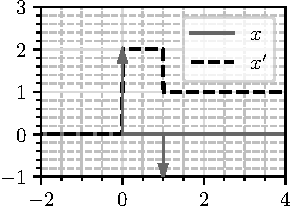
\includegraphics[scale=1]{fig/crtaj_ct_a.pdf}
        \caption{}
    \end{subfigure}
    \hspace*{0pt}\hfill
    \begin{subfigure}[c]{0.45\textwidth}
        \centering
        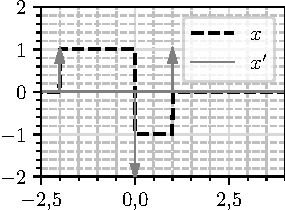
\includegraphics[scale=1]{fig/crtaj_ct_b.pdf}
        \caption{}
    \end{subfigure}
    \hfill
    \hspace*{0pt}

    \hspace*{0pt}\hfill
    \begin{subfigure}[c]{0.45\textwidth}
        \centering
        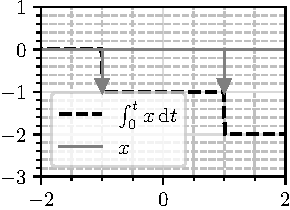
\includegraphics[scale=1]{fig/crtaj_ct_v.pdf}
        \caption{}
    \end{subfigure}
    \hspace*{0pt}\hfill
    \begin{subfigure}[c]{0.45\textwidth}
        \centering
        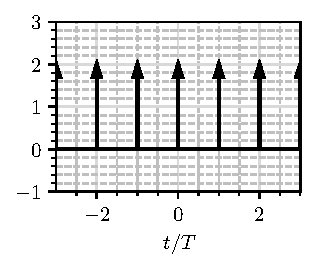
\includegraphics[scale=1]{fig/crtaj_ct_g.pdf}
        \caption{}
    \end{subfigure}
    \hfill
    \hspace*{0pt}

    \caption{}
\end{figure}